\section{Ziel}
Ziel des Versuches ist die Untersuchung des Rutherfordschen Streuexperimentes,
also die Streuung von Alpha-Teilchen an einer Goldfolie.

\section{Theorie}
\subsection{Alphastrahlung}
Der Begriff der Strahlung wird in Teilchen- und Wellenstrahlung unterteilt. Dabei
wird die Alphastrahlung der Teilchenstrahlung zugeordnet, da der zerfallende
Kern ein Helium-4-Atomkern absondert. Dieser Prozess ist durch den quantenmechanischen
Tunneleffekt zu erklären. Alphateilchen sind positiv geladen und verfügen über
eine schwere Masse, die die Abschirmung vereinfacht. \cite{potsdam}

\subsubsection{Wechselwirkung mit Materie}
Durchläuft ein Alphateilchen eine Materieschicht so erfährt es durch
Wechselwirkung mit den Hüllenelektron der Atome einen Energieverlust. Dieser
Energieverlust kommt durch Ionisation oder Anregung auf Grund von inelastischen
Stößen zustande. Die Flugrichtung der Alphateilchen erfährt daruch keine
Änderung. Die Bethe-Bloch Gleichung \eqref{eqn:bloch} beschreibt dabei den
Energieverlust pro Wegsträcke des Alphateilchens.

\begin{equation}
- \frac{\symup{d} E}{\symup{d} x} = \frac{4 \pi \symup{e}^4 z^2 \text{N} \text{Z}}
{\text{m}_0 v^2 (4 \pi \epsilon_0)^2} \ln\frac{2 \text{m}_0 v^2}{\text{I}}
\label{eqn:bloch}
\end{equation}
Die verwendeten Parameter sind die Anzahl der Atome pro \SI{}{\centi\meter\cubic}
N , die Kernladungszahl Z, die Geschwindigkeit v des Ions, die mittlere
Ionisationsenergie I und die Ruhemasse eines Elektrons $\text{m}_0$.
Gleichung \eqref{eqn:bloch} ist eine genäherte Version der Bethe-Bloch-Gleichung
und gilt für sehr kleine Teilchengeschwindigkeiten. Sie kann unter einigen
Annahmen aufgestellt werden. Eine davon lautet, dass ein geladenes, schweres
Teilchen an einem Elektron des Absorbermaterials in einem Abstand vorbei laufen
muss. Das Elektron ist dabei frei und bewegt sich kaum während der Wechselwirkung
mit dem Teilchen. Weiterhin gilt, dass die Masse des Teilchens sehr viel größer
als die Masse eines Elektrons sein muss.
\\
Eine weitere Wechselwirkung mit der Materie ist die durch Rutherford beschriebene
Streuung, die Hauptbestandteil dieses Experiments sein soll.

\subsection{Die Rutherford-Streuung}
Das Rutherfordsche Streuexperiments beschreibt die Ablenkung eines Alphateilchens
an Goldfolie. Diese Ablenkung kann zu einem durch einen elastischen Stoß mit
dem Kern des Absorbermaterials als auch durch das Coulombpotential von diesem
entstehen. Die Rutherfordsche Streuformel\eqref{eqn:streu} beschreibt diese Streuung.

\begin{equation}
  \frac{\symup{d} \sigma}{\symup{d} \Omega} (\Theta) =
  \frac{1}{(4 \pi \epsilon_0)^2} \left(\frac{\text{z} \text{Z} \symup{e}^2}
  {4 \text{E}_\alpha}\right)^2 \frac{1}{\sin^4\left(\frac{\Theta}{2}\right)}
  \label{eqn:streu}
\end{equation}

Der differentielle Wirkungsquerschnitt $\frac{\symup{d} \sigma}{\symup{d} \Omega} (\Theta)$
beschreibt den Winkel des gestreuten Teilchens pro Raumwinkelelement. Neben den
bei der Bethe-Bloch-Gleichung genannten Parametern wird hier zwischen der
Kernladung z des Alphateilchens und der Kernladung Z des Atoms unterschieden.
Weitere Parameter sind die mittlere kinetische Energie $\text{E}_\alpha$ des
Alphateilchens in \SI{}{\mega\electronvolt} und der Winkel $\Theta$ zwischen
einfallendem und gestreutem Alphateilchen.

\subsubsection{Konsequenzen des Streuversuches}
Die Entdeckung der Rutherford-Streuung hat große Auswirkung auf das damalige
Verständis des Atommodells. Das damalige Modell, das Thomsonsche Atommodell oder
auch Rosinenkuchenmodell genannt, besagte, dass die Elektronen in einem
positiv geladenen Atom eingebettet sind. Aus dem Rutherfordschen Streuexperiment
lässt sich jedoch die Schlussfolgerung ziehen, dass ein Atom ein positiven
Kern besitzt, auf dem sich fast die komplette Masse des Atoms konzentriert. Der
Kernradius muss zudem klein im Vergleich zum Atomradius sein. Somit wurde auf
Grund der Entdeckung von Rutherford ein neues Atommodell aufgestellt.

\subsection{241-Americium als Alphastrahler}
Der in diesem Versuch verwendete Alphastrahler ist 241-Americium. Er hat eine
Halbwertszeit von 432 a und eine Kernladungszahl von 95. Das Tochternuklid
ist 237-Neptunium. Es gibt fünf verschiedene Möglichkeiten wie 241-Americium in
sein Tochternuklid zerfallen kann \ref{fig:amnp}.

\begin{figure}[H]
  \centering
  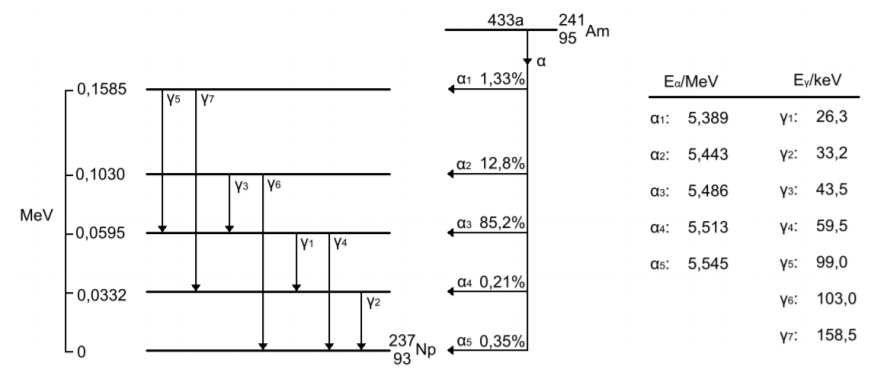
\includegraphics[width=\textwidth]{zerfall.png}
  \caption{Zerfallsmöglichkeiten von 241-Am  \cite{potsdam}.}
  \label{fig:amnp}
\end{figure}

Es ist zu erkennen, dass $\alpha_3$ der Wahrscheinlichste Zerfall ist. Der Zerfall
von Neptunium ist in diesem Fall nicht mehr relevant, da dessen Halbwertszeit
sehr groß im Vergleich zu Americium ist.
